% Options for packages loaded elsewhere
\PassOptionsToPackage{unicode}{hyperref}
\PassOptionsToPackage{hyphens}{url}
\documentclass[12pt, ]{article}

\usepackage{mathtools}
\usepackage{amsmath}
\usepackage{amsthm}
\usepackage{amssymb}
\usepackage[italicdiff]{physics}
\mathtoolsset{showonlyrefs}

% SPACING AND FONTS %%%%%%%%%%%%%%%%%%%%%%%%%%%%%%%%%%%%%%%%%%%%%%%%%%%%%%%%%%%%
\usepackage{iftex}
% CAREFUL: the order of font includes here is very important!
\ifPDFTeX
  \usepackage[OT1,T1]{fontenc}
  \usepackage[utf8]{inputenc}
  \usepackage{textcomp} % provide euro and other symbols
    \usepackage[p,osf,swashQ]{cochineal}
  \usepackage[cochineal,vvarbb]{newtxmath}
      \usepackage[scale=0.95]{biolinum}
    \usepackage[scale=0.95,varl]{inconsolata}
\else % if luatex or xetex
  \usepackage[scale=0.95,varl]{inconsolata}
  \usepackage{newpxtext}
  \usepackage{mathpazo}
    \usepackage[scale=0.95]{biolinum}
  \fi
\ifLuaTeX
  \usepackage{selnolig}  % disable illegal ligatures
\fi
\IfFileExists{microtype.sty}{% use microtype if available
  \usepackage[]{microtype}
  \UseMicrotypeSet[protrusion]{basicmath} % disable protrusion for tt fonts
}{}

\setlength{\parindent}{0pt}
\setlength{\parskip}{10pt plus 2pt minus 2pt}
\setlength{\emergencystretch}{3em} % prevent overfull lines
\widowpenalty=10000
\clubpenalty=10000
\flushbottom
\allowdisplaybreaks
\sloppy


% CORE PACKAGES %%%%%%%%%%%%%%%%%%%%%%%%%%%%%%%%%%%%%%%%%%%%%%%%%%%%%%%%%%%%
\usepackage[dvipsnames,svgnames,x11names]{xcolor}
\usepackage[lmargin=1.5in,rmargin=1.5in,tmargin=1.2in,bmargin=1.2in]{geometry}
\usepackage[format=plain,
  labelfont={bf,sf,small,singlespacing},
  textfont={sf,small,singlespacing},
  justification=justified,
  margin=0.25in]{caption}

% SECTIONS AND HEADINGS %%%%%%%%%%%%%%%%%%%%%%%%%%%%%%%%%%%%%%%%%%%%%%%%%%%%%%%%
\setcounter{secnumdepth}{4}
\usepackage{sectsty}
\usepackage[compact]{titlesec}
% short title
\makeatletter
\newcommand\@shorttitle{}
\newcommand\shorttitle[1]{\renewcommand\@shorttitle{#1}}
\usepackage{fancyhdr}
\fancyhf{}
\pagestyle{fancy}
\renewcommand{\headrulewidth}{0pt}
\fancyheadoffset{0pt}
%\lhead{\scshape \@shorttitle}
%\rhead{\scshape\today}
\cfoot{\thepage}
\makeatother
% abstract styling
\renewenvironment{abstract}{
  \centerline
  {\large\sffamily\bfseries Abstract}\vspace{-1em}
  \begin{quote}\small
}{
  \end{quote}
}

% PANDOC INCLUDES %%%%%%%%%%%%%%%%%%%%%%%%%%%%%%%%%%%%%%%%%%%%%%%%%%%%%%%%%%%%%%

\providecommand{\tightlist}{%
  \setlength{\itemsep}{0pt}\setlength{\parskip}{0pt}}\usepackage{longtable,booktabs,array}
\usepackage{calc} % for calculating minipage widths
% Correct order of tables after \paragraph or \subparagraph
\usepackage{etoolbox}
\makeatletter
\patchcmd\longtable{\par}{\if@noskipsec\mbox{}\fi\par}{}{}
\makeatother
% Allow footnotes in longtable head/foot
\IfFileExists{footnotehyper.sty}{\usepackage{footnotehyper}}{\usepackage{footnote}}
\makesavenoteenv{longtable}
\usepackage{graphicx}
\makeatletter
\def\maxwidth{\ifdim\Gin@nat@width>\linewidth\linewidth\else\Gin@nat@width\fi}
\def\maxheight{\ifdim\Gin@nat@height>\textheight\textheight\else\Gin@nat@height\fi}
\makeatother
% Scale images if necessary, so that they will not overflow the page
% margins by default, and it is still possible to overwrite the defaults
% using explicit options in \includegraphics[width, height, ...]{}
\setkeys{Gin}{width=\maxwidth,height=\maxheight,keepaspectratio}
% Set default figure placement to htbp
\makeatletter
\def\fps@figure{htbp}
\makeatother
% END PANDOC %%%%%%%%%%%%%%%%%%%%%%%%%%%%%%%%%%%%%%%%%%%%%%%%%%%%%%%%%%%%%%%%%%%

% USER INCLUDES %%%%%%%%%%%%%%%%%%%%%%%%%%%%%%%%%%%%%%%%%%%%%%%%%%%%%%%%%%%%%%%%
% additional LaTeX code for the "preamble" goes here
\makeatletter
\makeatother
\makeatletter
\makeatother
\makeatletter
\@ifpackageloaded{caption}{}{\usepackage{caption}}
\AtBeginDocument{%
\ifdefined\contentsname
  \renewcommand*\contentsname{Table of contents}
\else
  \newcommand\contentsname{Table of contents}
\fi
\ifdefined\listfigurename
  \renewcommand*\listfigurename{List of Figures}
\else
  \newcommand\listfigurename{List of Figures}
\fi
\ifdefined\listtablename
  \renewcommand*\listtablename{List of Tables}
\else
  \newcommand\listtablename{List of Tables}
\fi
\ifdefined\figurename
  \renewcommand*\figurename{Figure}
\else
  \newcommand\figurename{Figure}
\fi
\ifdefined\tablename
  \renewcommand*\tablename{Table}
\else
  \newcommand\tablename{Table}
\fi
}
\@ifpackageloaded{float}{}{\usepackage{float}}
\floatstyle{ruled}
\@ifundefined{c@chapter}{\newfloat{codelisting}{h}{lop}}{\newfloat{codelisting}{h}{lop}[chapter]}
\floatname{codelisting}{Listing}
\newcommand*\listoflistings{\listof{codelisting}{List of Listings}}
\makeatother
\makeatletter
\@ifpackageloaded{caption}{}{\usepackage{caption}}
\@ifpackageloaded{subcaption}{}{\usepackage{subcaption}}
\makeatother
\makeatletter
\@ifpackageloaded{tcolorbox}{}{\usepackage[skins,breakable]{tcolorbox}}
\makeatother
\makeatletter
\@ifundefined{shadecolor}{\definecolor{shadecolor}{rgb}{.97, .97, .97}}
\makeatother
\makeatletter
\makeatother
\makeatletter
\makeatother
% END USER INCLUDES %%%%%%%%%%%%%%%%%%%%%%%%%%%%%%%%%%%%%%%%%%%%%%%%%%%%%%%%%%%%

% BIBLIOGRAPHY %%%%%%%%%%%%%%%%%%%%%%%%%%%%%%%%%%%%%%%%%%%%%%%%%%%%%%%%%%%%%%%%%
\usepackage[]{natbib}
\bibliographystyle{apalike}

% Give it this name so that it works with ::: #refs
\newenvironment{CSLReferences}[2]{
\bibliography{bibliography.bib}
\clearpage
}{}

% LINKS %%%%%%%%%%%%%%%%%%%%%%%%%%%%%%%%%%%%%%%%%%%%%%%%%%%%%%%%%%%%%%%%%%%%%%%%
\usepackage{hyperref}
\usepackage{url}
\hypersetup{
  pdftitle={On the Fast Train: Seeking Political Incentives for High-Speed Rail Construction in China},
  pdfauthor={Daevan Mangalmurti},
  colorlinks=true,
  linkcolor={black},
  filecolor={Maroon},
  citecolor={VioletRed4},
  urlcolor={DodgerBlue4},
  pdfcreator={LaTeX via pandoc}}

% TITLE, AUTHOR, DATE %%%%%%%%%%%%%%%%%%%%%%%%%%%%%%%%%%%%%%%%%%%%%%%%%%%%%%%%%%
\title{\sffamily\bfseries\huge\parfillskip=0pt
\rightskip=0pt plus .5\textwidth
\leftskip=0pt plus .5\textwidth
\emergencystretch=.3\textwidth On the Fast Train: Seeking Political
Incentives for High-Speed Rail Construction in China}
\shorttitle{On the Fast Train: Seeking Political Incentives for High-Speed Rail Construction in China}
\author{\textbf{Daevan Mangalmurti}
 }
\date{}


\begin{document}
\allsectionsfont{\sffamily}

\maketitle

\begin{abstract}
Recent work on China's infrastructure has argued that politicians are
motivated to build long-term projects by short-term career goals. Using
original data on high-speed rail infrastructure, I examine the
relationship between high-speed rail, economic performance, and
politicians' promotion. I do not find evidence of a significant
relationship between high-speed rail approval and promotion rates, and
suggest that further work is necessary to illuminate incentives for
infrastructure development.
\end{abstract}

\ifdefined\Shaded\renewenvironment{Shaded}{\begin{tcolorbox}[boxrule=0pt, sharp corners, borderline west={3pt}{0pt}{shadecolor}, breakable, frame hidden, interior hidden, enhanced]}{\end{tcolorbox}}\fi



% USER BODY %%%%%%%%%%%%%%%%%%%%%%%%%%%%%%%%%%%%%%%%%%%%%%%%%%%%%%%%%%%%%%%%%%%%

\hypertarget{introduction}{%
\section{Introduction}\label{introduction}}

Building infrastructure, like all types of public goods provision,
demands political choices. These may be driven by personal priorities,
as when a politician with a two-year term builds a project that will be
done by reelection rather than a road requiring a decade. Choices may
respond to perceived needs, as when a politician decides which
neighborhood should have its roads repaired first. A core function of
political science is studying public goods provision to understand who
gets what, and why. Examining distributive politics is the path toward
ensuring that government services meet public needs. The bigger the
scale of a public good, the more urgent it is to understand the
incentives governing its allocation.

In this century, China has built more infrastructure, faster, than any
other country \citep{OECD2023}. Its infrastructure spending represents
almost 1\% of global GDP. China's success defies the mismatch between
short-term political incentives and long-term infrastructure demands
that confronts most countries.

How has China done it? In ``Private Returns to Public Investment:
Political Career Incentives and Infrastructure Investment in China,''
Lei and Zhou argue that one answer lies in China's political structure
\citep{lei_private_2022}. Unlike in democracies, where politicians
answer to voters, Chinese politicians answer to their superiors. This
reduces the electoral costs of building infrastructure and aligns
short-term and long-term interests. Provincial Chinese politicians are
charged by the central government with delivering economic growth. When
prefectural politicians---mayors and party secretaries---produce
economic results---e.g.~by investing in infrastructure---they are
demonstrating their competence, but also helping provincial politicians
fulfill their mandates. In doing so, they may increase their chances of
being promoted. This theory is supported by a growing body of work
linking economic performancew with political advancement in China
\citep{luo_chinas_2021, landry_does_2018}

Using an original dataset on subway approvals, Lei and Zhou demonstrate
that mayors who receive approval to build subways have higher promotion
rates than mayors overall. They show that the mechanism for this
relationship is likely an increase in economic performance after a
subway is approved. A better economy signals helpfulness and contributes
to a provincial politicians' objectives \citep{lei_private_2022}.

In this paper, I apply Lei and Zhou's theory of incentives to a
different kind of infrastructure: high-speed rail (HSR). Like subways,
HSR is perceived as a contributor to economic growth and a desirable
form of infrastructure for cities. This makes it well-suited to testing
(a) whether there is a relationship between infrastructure beyond
subways and prefectural officials' promotion and (b) whether the
presence or absence of that relationship is due to the mechanism of
economic performance.

Using an original dataset on Chinese cities' HSR approvals, I study the
relationship between HSR and prefectural officials' promotion. Using a
differences-in-differences identification strategy, I find that there is
not a significant positive relationship between a city receiving
approval for HSR and politicians' likelihood of promotion for either
mayors or party secretaries. I demonstrate that a likely reason for the
absence of a positive relationship in my dataset is the absence of Lei
and Zhou's proposed mechanism. There is not a consistently positive
relationship between high-speed rail approval and local economic
outcomes. I suggest that this shows that Lei and Zhou's theory is useful
but does not explain why HSR has been and continues to be built, and I
conclude by explaining the next stage of my research on this topic.

\hypertarget{background-high-speed-rail-in-china}{%
\section{Background: High-Speed Rail in
China}\label{background-high-speed-rail-in-china}}

In the decade to 2019, China built 25,000 kilometers of HSR, more than
any other country's existing HSR network \citep{lawrence_chinas_2019}.
The process for constructing a high-speed rail line can be divided into
four general phases \citep{ma_localized_2022}.

The process begins at the local level, where local governments prepare
proposals and submit them to China Railway Corporation (CRC), the
state-owned railway company. If CRC, the Ministry of Transport, and the
National Development and Reform Commission (NDRC) agree that the
proposed route should be considered, it is included in one of the
Five-Year Plans in the Medium- and Long-Term Railway Plan (MLTRP), the
central government's comprehensive 15-year HSR plan
\citep{ma_localized_2022, lawrence_chinas_2019}.

The project now moves into pre-feasibility evaluation by the CRC. If the
proposal passes, CRC and the proposing government send it to the NDRC.
If the NDRC approves the proposal, that marks the central government's
formal acceptance of the project.

Once the proposal has been been accepted by the NDRC, it goes through
feasibility evaluations. These include review by the CRC, NDRC, and up
to five other ministries. During this period, the proposal is often
revised substantially to satisfy their requirements. Once all parties
are satisfied, the proposal, now called a ``project feasibility report''
is sent back to the NDRC for approval. The final phase, during which the
relevant local government begins preparing for construction, comes once
the project feasibility report is approved \citep{ma_localized_2022}.

The HSR network has widely been seen as the product of top-down efforts
by China's central government. While the central government sets targets
in terms of rail construction and oversees the operation of HSR routes,
the HSR approval process clearly shows that HSR is heavily dependent on
local government involvement. Recent work has shown that this is true to
a greater degree than previously thought. Cities will spend years
lobbying and negotiating with the central government for approval to
construct or extent HSR routes. This can extend to maintaining offices
in Beijing to push for a city's interests
\citep{ma_localized_2022, ji_revolutionaries_2022}.

Although central government approval is a prerequisite for building HSR,
the cost of a dedicated HSR station---a requirement for most Chinese
cities' initial HSR lines---and land acquisition is mostly borne by
local governments
\citep{yang_wrestling_2020, yuan_peer_2023, wang_unravelling_2021}.
Route operations are also partially subsidized by the local
government---an issue because many HSR lines lose money
\citep{ma_localized_2022}. The fact that governments lobby for
permission to build HSR nonetheless demonstrates that HSR is perceived
as having significant benefits. Studies of HSR development in Chinese
cities has found that the siting of HSR lines has been used to try to
shift cities' economic centers of gravity
\citep{wang_planning_2022, chen_change_2021, zhu_does_2021, chi_impact_2023};
to decrease travel times with the aim of improving connectivity and
economic synergy
\citep{huang_intercity_2022, lawrence_chinas_2019, xu_planning_2014};
and to increase investment and revenue
\citep{wang_planning_2022, yang_wrestling_2020}. While productivity
gains from reduced travel time are well-documented, the actual economic
benefits are not. Studies have found evidence that HSR construction
leads to changes in urbanization patterns and that housing and land near
HSR stations increases in value
\citep{wang_planning_2022, yang_wrestling_2020}. Globally, HSR has been
shown to increase local GDP growth through greater connectivity, but it
has also been found to negatively affect peripheral regions and
industrial areas by concentrating labor and capital in hub cities
\citep{chi_impact_2023, zhu_does_2021}. Recent work on China has also
found that cities that build HSR experience increases in their financing
costs for other projects
\citep{ruan_high-speed_2023, yuan_chinas_2023, JianZhao2019}.

All of this indicates that while HSR is regarded as a net economic boon,
its actual effect may be more mixed at the local level. At the
provincial level, higher connectivity should result in higher GDP growth
and per capita GDP. The fact that local governments continue to lobby
for and build HSR lines indicates that, similar to subway lines, HSR has
large perceived economic benefits. Since HSR routes are often finished
after the term of the prefectural officials under whom they were
started, HSR is therefore a useful test of Lei and Zhou's theory that
investing in infrastructure signals ``helpfulness'' to provincial
leaders and can show whether that relationship holds even for projects
with mixed economic consequences at the local level but positive
provincial outcomes.

\hypertarget{data}{%
\section{Data}\label{data}}

I rely on two datasets for my empirical analysis. I begin by collecting
an original dataset of 103 observations on intercity high-speed rail
construction between 2003 and 2022. Intercity high-speed rail includes
regional HSR lines with speeds of 200-350 km/h. I focus on intercity
railways because they require the greatest involvement from local
governments. Like all HSR lines, intercity lines are approved by the
central government, but they receive more significant financing from
local governments than national HSR, and their day-to-day operations are
more highly subsidized by cities. As such, intercity HSR requires high
levels of initiative and lobbying from local governments. If
infrastructure investment is used to generate economic growth and signal
helpfulness and competence, HSR should provide the closest analogue to
Lei and Zhou's subway dataset and therefore be a useful test of the
applicability of their incentive theory to other infrastructure
projects.

I collect the names and routes of intercity HSR projects from Wikipedia
\footnote{https://en.wikipedia.org/wiki/List\_of\_high-speed\_railway\_lines\_in\_China.}.
Where it is publicly available, I use the year in which the NDRC
approved a route's project feasibility report as the year of approval.
Otherwise I use the year in which construction began. In many cases
construction begins in the same year as approval, so I do not lag the
year in which construction began to find approval. One exception to this
was HSR in Tangfang and Langshan, which was approved in 2009 but did not
start until 2015 \footnote{Reported in the \emph{Beijing Daily},
  http://bj.people.com.cn/n2/2015/1230/c82840-27429354.html and
  bj.people.com.cn/n2/2015/1230/c82840-27429354.html.}. I use 2009 as
the year of approval and, following Lei and Zhou, would expect to see
economic effects soon after approval was announced. When I run my
identification strategy on lagged data I do not find any changes in the
significance of the relationship between HSR approval and promotion.

The rest of the data used in this paper comes from Lei and Zhou (2022),
who collect data on prefectural and provincial officials' promotion
demographics and promotion rates, cities' performance on a range of
economic indicators, and subway approval from the China Association of
Metros, CCER Official Dataset, Chinese Political Elite Database, Chinese
City Statistical Yearbook, and China Urban Construction Statistical
Yearbook. I follow Lei and Zhou in dropping 15 vice-provincial level
cities from my dataset because of their different promotion processes
compared to normal prefectural cities \citep{lei_private_2022}. These
cities are Guangzhou, Wuhan, Harbin, Shenyang, Chengdu, Nanjing, Xi'an,
Changchun, Jinan, Hangzhou, Dalian, Qingdao, Shenzhen, Xiamen, and
Ningbo.

\hypertarget{methodology}{%
\section{Methodology}\label{methodology}}

My primary identification strategy uses a difference-in-difference
approach. My regression specification is of the following form:
\[Promotion_{pit} = \beta_{0} + \beta_{1}{HSR Approval}_{i,t} + \gamma X_{i,t - 1} + \theta_{i} + \pi_{t} + \varepsilon_{it}.\]
My outcome variable is the variable \(Promotion_{pit}\), which indicates
whether a prefectural official from city \(i\) is promoted within three
years of year \(t\), the year of HSR approval. The index \(p\) indicates
whether the official in question is a mayor or a party secretary. I
follow Lei and Zhou in defining a mayor's promotion as promotion to
``party secretary of a prefecture-level city or a vice-province-level
position.'' A party secretary's promotion is promotion to a
province-level party secretary position. Since the both mayors and party
secretaries serve for an average of three years, promotion is within
three years.

\begin{table}
  \caption{Summary Statistics}
  \label{Table1}
  \begin{longtable}{lrrrr}
\toprule
Variable & N & Mean & Min & Max \\ 
\midrule
Mayor promoted within three years & $3,843$ & $0.41$ & $0.00$ & $1.00$ \\ 
Party secretary promoted within three years & $3,829$ & $0.17$ & $0.00$ & $1.00$ \\ 
High-speed rail project approved & $3,861$ & $0.03$ & $0.00$ & $3.00$ \\ 
City population & $3,571$ & $417.42$ & $14.19$ & $1,591.76$ \\ 
City GDP (billion ¥) & $3,852$ & $135.57$ & $3.18$ & $1,954.74$ \\ 
City fiscal revenue (billion ¥) & $3,856$ & $10.39$ & $0.12$ & $313.65$ \\ 
City investment in infrastucture per capita (¥) & $3,848$ & $699.33$ & $0.00$ & $13,236.19$ \\ 
City GDP per capita (¥) & $3,845$ & $32,218.63$ & $99.00$ & $467,749.00$ \\ 
City land sales revenue per capita (¥) & $3,855$ & $296.91$ & $0.00$ & $40,277.59$ \\ 
City fiscal revenue per capita (¥) & $3,855$ & $2,697.62$ & $70.33$ & $81,467.34$ \\ 
\bottomrule
\end{longtable}


  \caption*{Summary stats for rows 1 and 4-10 replicate Table 1 in Lei and Zhou 2022.}
\end{table}

Receiving HSR approval is a long-term process that requires involvement
from both a city's mayor and its party secretary. There is no definitive
way beyond intensive qualitative interviews of determining which
official in a given city may have been responsible for securing
approval. As such, I use a generalized treatment variable,
\(HSR Approval_{it}\) that equals 1 if a city, \(i\) has been approved
for an HSR line in year \(t\), and 0 otherwise.

My regression equation uses a vector of city control variables that
includes the time variant characteristics of a city: population, GDP
growth, gdp per capita, and annual revenue. I lag these variables by one
year to avoid post-treatment effects. Depending on the outcome variable
in question, I also control for mayors' characteristics or party
secretaries' characteristics. Finally, I include fixed effects for the
city, \(\theta_{i}\) and year, \(\pi_{t}\). I report standard errors
clustered at the city level.

In addition to my baseline identification strategy, I test a fuzzy
regression discontinuity approach to assessing the relationship between
promotion and HSR approval. The problem this approach faces is that
there is no well-defined cutoff in my data between cities that are
eligible for HSR and those that are not. Through the 2010s, the
objective of Chinese central government policy was to ensure that all
cities with populations above 1 million were connected via HSR. There
are practically no cities in my dataset with populations below 1
million. Instead, I run a fuzzy RD model at city populations of 3
million, the same cutoff used for subway approval by Lei and Zhou. This
approach faces sorting issues and I do not report the results over
concerns over the validity of the approach and wildly varying
coefficient estimates. The results can be found in the appendix.

Finally, after running my initial identification strategy, I turn to
investigating the economic performance mechanism proposed by Lei and
Zhou. For each of the indicators of economic performance I use, I use an
equation of the following form:
\[Indicator_{it} = {HSR Approval}_{i, t + n} + \gamma X_{i,t + n} + \theta_{i} + \varepsilon_{it}.\]
The outcome variable is an indicator of one of five measures of economic
performance: infrastructure investment, per capita GDP, per capita
revenue from land sales, annual revenue per capita, and the unemployment
rate. I regress the outcome variable on the treatment variable,
\(HSR Approval\), lagged and lead up to five years in either direction
(represented by \(n\). My control variables are city characteristics,
mayor characteristics, and party secretary characteristics. I include
city fixed effects.

\hypertarget{results}{%
\section{Results}\label{results}}

Table 2 shows the results of my baseline difference in difference
analysis. The outcome variable is promotion within three years for both
mayors and party secretaries.

Model (1) regresses the outcome variable on approval of an HSR plan
during a mayor's term and includes city and year fixed effects. Model
(2) regresses the outcome variable on approval of an HSR plan during a
mayor's term and adds controls for the mayor's characteristics,
including gender, ethnicity, age education, political connection with
provincial party secretary, and previous work experience in county
government, provincial government, central government, state-owned
enterprises, university, and the Communist Youth League. Model (3) adds
controls for the city's population, GDP, fiscal revenue, and GDP growth
in the previous year (to avoid reporting post-treatment effects). Model
(4) adds province-year fixed effects.

\begin{table}
  \centering
  \caption{Regression Table}
  \label{Table2}
  \begin{longtable}{lcccccccc}
\caption*{
{\large HSR Approval and Prefectural Official Promotion} \\ 
{\small Promotion within three years}
} \\ 
\toprule
 & \multicolumn{4}{c}{Mayor} & \multicolumn{4}{c}{Party Secretary} \\ 
\cmidrule(lr){2-5} \cmidrule(lr){6-9}
  & (1) & (2) & (3) & (4) & (5) & (6) & (7) & (8) \\ 
\midrule
HSR\_Approval & -0.006 & 0.000 & -0.003 & -0.057 & 0.024 & 0.025 & 0.034 & -0.002 \\ 
 & (0.045) & (0.045) & (0.048) & (0.056) & (0.028) & (0.027) & (0.030) & (0.039) \\ 
Num.Obs. & 3843 & 3761 & 3247 & 3247 & 3829 & 3661 & 3165 & 3165 \\ 
FE: City\_Code & X & X & X & X & X & X & X & X \\ 
Year FE & X & X & X & X & X & X & X & X \\ 
Province-year FE &  &  &  & X &  &  &  & X \\ 
\bottomrule
\end{longtable}


  \caption*{Standard errors in parentheses are clustered at the city level. Mayor controls are: gender, ethnicity, age, education, political connection with provincial party secretary, and previous work experiences. Party secretary controls are: gender, ethnicity, age, education, political connection with provincial party secretary, and previous work experiences. City controls are population, GDP, fiscal revenue, and GDP growth rate in the previous year. FE means fixed effects. Mayor and city control variables are taken from Lei and Zhou 2022.}
\end{table}

The table shows that there is not a significant relationship, or much of
a relationship at all, between mayors' promotion and a city receiving
HSR approval during their term. Model (4) finds that HSR approval
decreases mayors' promotion chances by 5.7 percentage points, but this
is still not significant. The absence of a relationship between HSR
approval and mayors' promotion remains true when the outcome variable is
changed to promotion within five, four, or two years. In the appendix
(Table 2A), I show that for the first three models, there is a small but
slightly significant negative relationship between a mayor's promotion
chances within one year and HSR approval when approval is lagged by two
years, with a coefficient range of -5.6 to -6.2 percentage points, which
would suggest that HSR construction two years prior to the year in
question decreases a mayor's chances of promotion in that year by 5.6 to
6.2 percentage points. This effect disappears in model four. I interpret
that finding as suggesting that mayors coming into a city that has
already had HSR approval face greater difficulty in getting promoted,
either because there are fewer large infrastructure projects they can
use to demonstrate their competence and helpfulness, or because HSR
worsens a city's economic condition through the negative effects on
financing costs described by Ruan et al.~2023.

Models (5) through (8) follow the same specifications as models (1)
through (4), but with party secretary promotion within three years as
the outcome variable and controlling for party secretaries' gender,
ethnicity, age education, political connection with provincial party
secretary, and previous work experience in county government, provincial
government, central government, state-owned enterprises, university, and
the Communist Youth League in models (6), (7), and (8). I find a small
and positive relationship between HSR approval and party secretaries'
promotion in models (5) through (7), but this turns negative in model
(8) and is not significant. Changing the timeline of the outcome
variable and lagging HSR approval leads to inconsistent flipping of
signs, but no significant results.

There is not a significant relationship, either positive or negative,
between HSR approval and prefectural officials' promotion. To
investigate why this might be, I examine the effects of HSR approval on
four indicators of economic performance: infrastructure investment, per
capita GDP, land sales revenue, and fiscal revenue, which I display in
Figure 1.

In Fig. 1a, I find that infrastructure investment rises in the years
immediately after a city receives HSR approval, then decreases
dramatically. This suggests that HSR approval does not yield significant
benefits to investment in infrastructure, possibly because financing HSR
construction makes it more difficult for cities to attract investment
for other projects by worsening their fiscal situations
\citep{ruan_high-speed_2023}. Fig. 1b finds no relationship between per
capita GDP and HSR approval, though the consistency of the 0 coefficient
and size of the standard error suggests that there may be issues in
calculating that relationship.

\begin{figure}[tbp]

{\centering 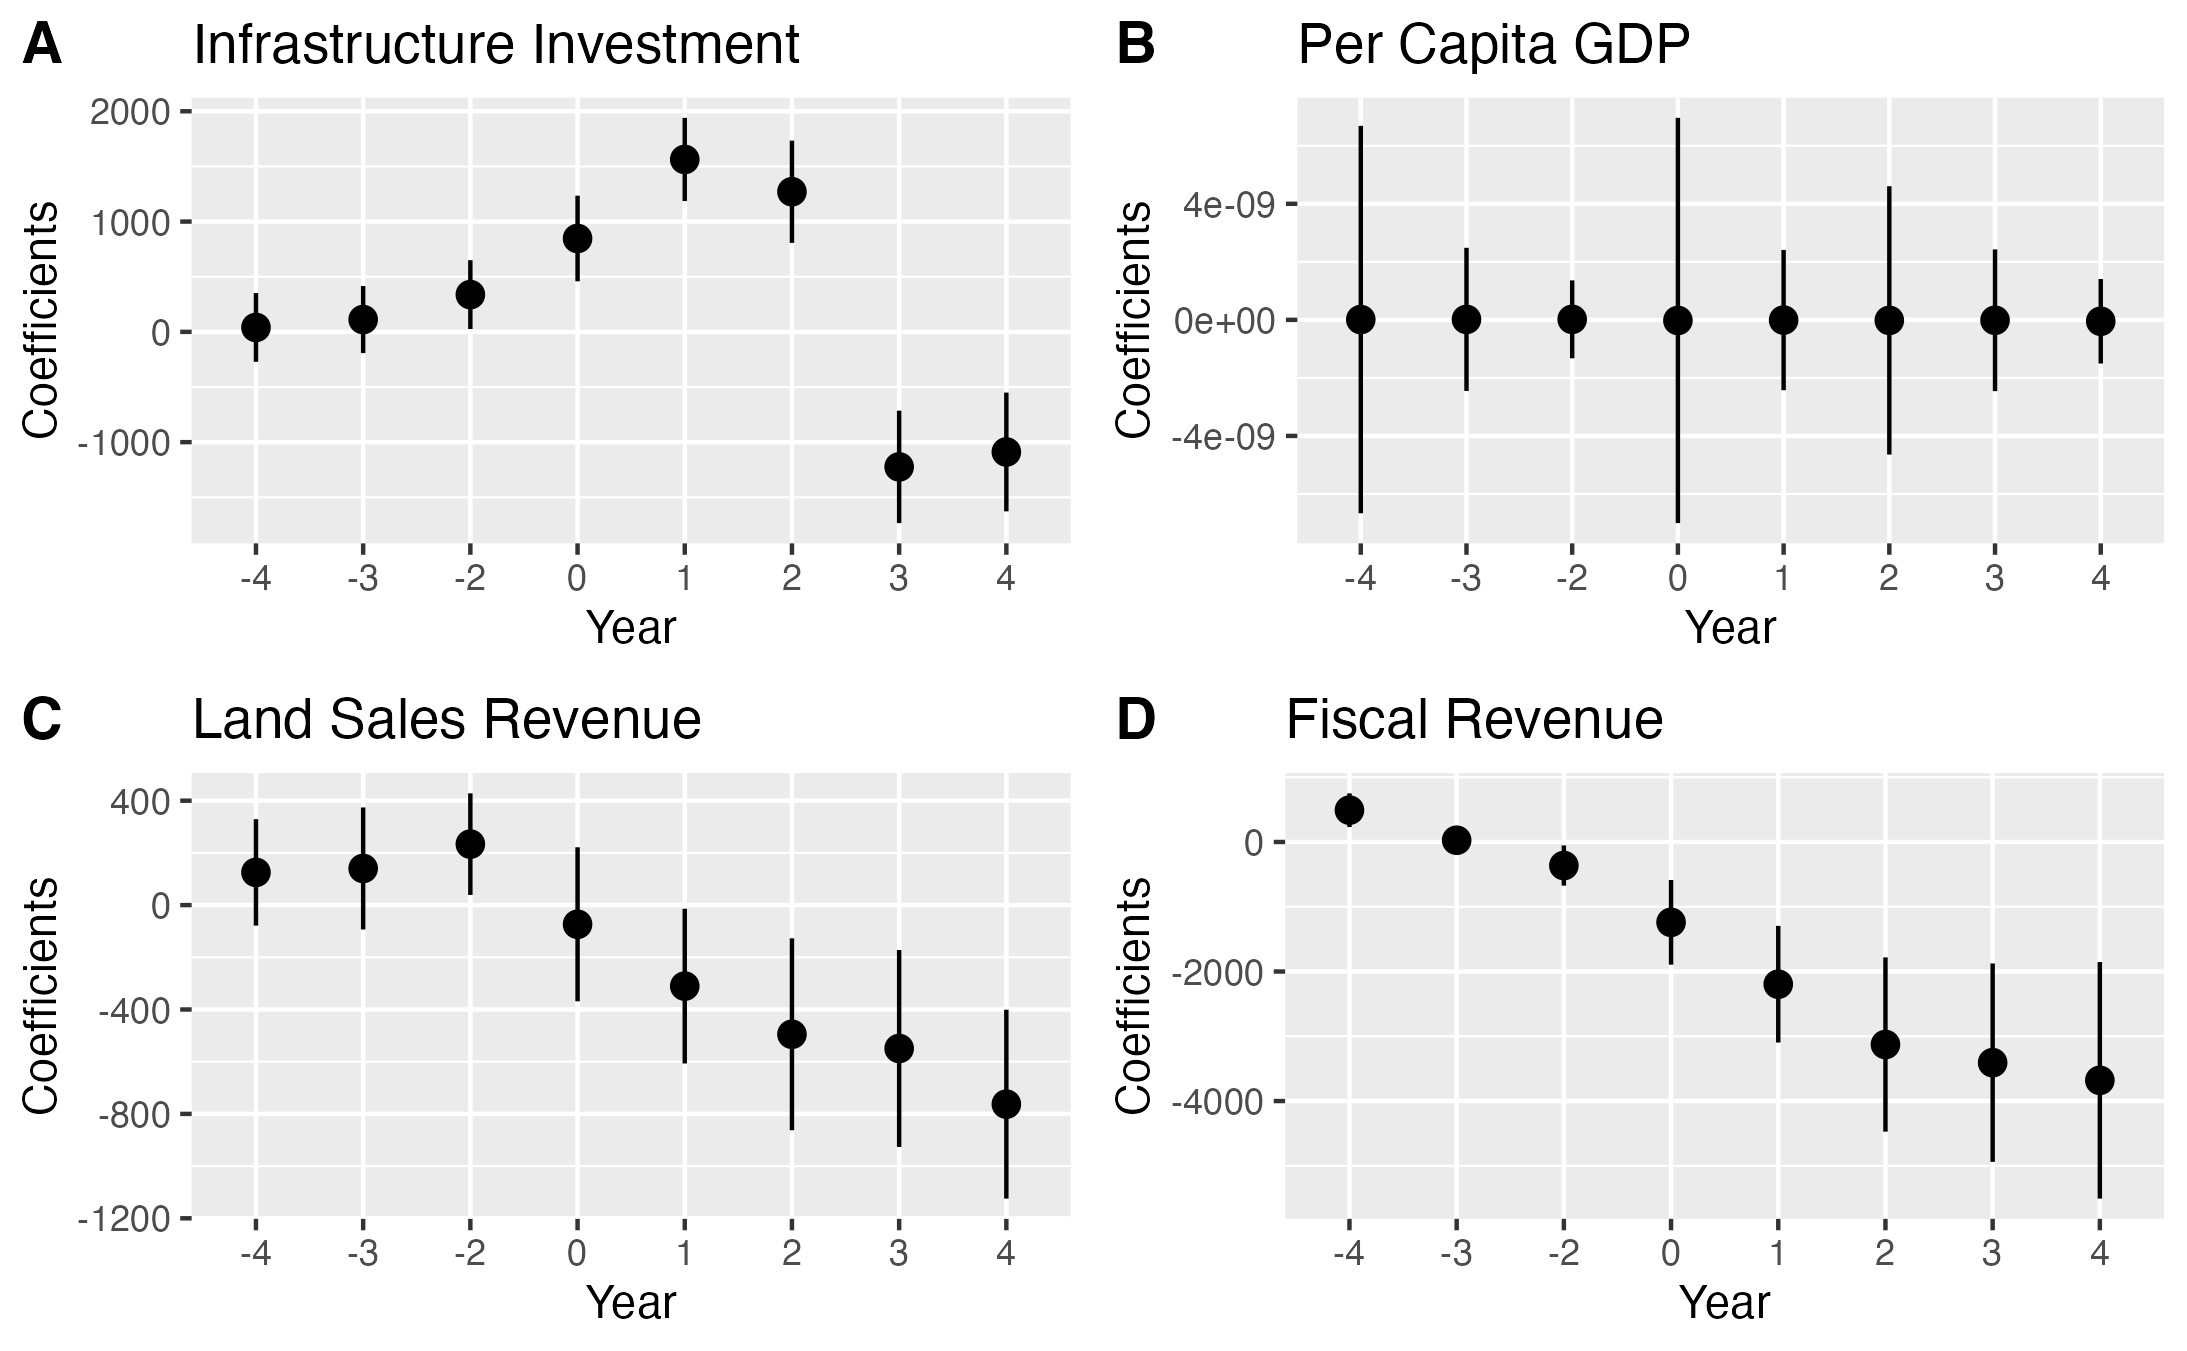
\includegraphics{figures/figure1_mech.png}

}

\caption{Dynamic Effects of HSR Approval on Economic Indicators}

\end{figure}

In Fig. 1c, I turn to land sales revenue, which cities earn by
auctioning land to private buyers (\citet{lei_private_2022}). I find
that land sales revenue declines each year after HSR approval, which is
contrary to prior findings (\citet{wang_planning_2022}) but may be
supported by the fact that cities provide land for the construction of
HSR lines and stations. In doing so, they may reduce the land available
for auctions and thereby decrease their land sales revenue. Finally, in
Fig. 1d I also find that fiscal revenue declines after HSR approval,
although this appears to be a continuation of pre-approval trends. This
finding is also surprising.

In sum, Fig. 1 shows that the mechanism linking long-term infrastructure
construction with short-term political incentives does not hold in the
case of HSR. HSR does not lead to improved economic performance, at
least in my sample. This helps explain why HSR approval is not linked to
higher chances of promotion in my difference-in-difference analysis.
Unlike subway approval, HSR approval is not an omen of stronger economic
performance, and therefore does not fulfill a signaling purpose for
prefectural officials' political superiors.

\hypertarget{conclusion}{%
\section{Conclusion}\label{conclusion}}

This study sought to determine whether prefectural officials in China
are motivated to construct high-speed rail infrastructure by the
prospect of economic benefits that lead to increased chances of
promotion. I find that there is not a relationship between HSR approval
and either officials' chances of promotion or their cities' economic
performance after approval. Despite this, high-speed rail continues to
be built across China. My results suggest that the explanation for why
politicians build HSR is not based on its economic and career benefits,
and that there is a different reason for seeking HSR lines and approval.
I plan to continue this study with an expanded dataset of HSR lines and
construction across China to determine if my results remain true and if
there is a different mechanism linking politicians' short-term interests
with their record of building long-term infrastructure.

\newpage{}

\hypertarget{refs}{}

\begin{CSLReferences}{0}{0}\end{CSLReferences}

\appendix

\hypertarget{appendix}{%
\section{Appendix}\label{appendix}}

\newpage{}

\begin{table}
  \centering
  \caption*{Table 1A: RD Regression Table}
  \label{Table1A}
  \begin{longtable}{lcccccc}
\toprule
  & (1) & (2) & (3) & (4) & (5) & (6) \\ 
\midrule
fit\_HSR\_Approval & 126.968 & -31.167 & 237.438 & -69.996 & 58.851 & -4.334 \\ 
 & (167.969) & (59.817) & (10253.638) & (97.103) & (173.537) & (10.987) \\ 
Per\_pop\_2 & 17.638 & -0.546 & -9.636 & -12.831 & -25.999 & 0.618 \\ 
 & (22.429) & (8.239) & (279.110) & (12.257) & (69.107) & (7.156) \\ 
iv1\_int & -16.050 & -0.750 & 13.873 & 11.555 & 24.517 & -0.332 \\ 
 & (23.775) & (8.180) & (457.474) & (12.964) & (66.116) & (6.423) \\ 
Num.Obs. & 534 & 523 & 518 & 536 & 523 & 518 \\ 
\bottomrule
\end{longtable}


\end{table}

\begin{table}
  \centering
  \caption*{Table 2A: Regression Table}
  \label{Table2A}
  \setlength{\LTpost}{0mm}
\begin{longtable}{lcccccccc}
\caption*{
{\large HSR Approval and Prefectural Official Promotion} \\ 
{\small Promotion within one year}
} \\ 
\toprule
 & \multicolumn{4}{c}{Mayor} & \multicolumn{4}{c}{Party Secretary} \\ 
\cmidrule(lr){2-5} \cmidrule(lr){6-9}
  & (1) & (2) & (3) & (4) & (5) & (6) & (7) & (8) \\ 
\midrule
lag(HSR\_Approval, n = 2) & -0.062** & -0.062** & -0.056* & -0.039 & 0.014 & 0.013 & 0.013 & 0.021 \\ 
 & (0.023) & (0.023) & (0.024) & (0.032) & (0.020) & (0.020) & (0.023) & (0.026) \\ 
Num.Obs. & 3843 & 3761 & 3247 & 3247 & 3829 & 3661 & 3165 & 3165 \\ 
FE: City\_Code & X & X & X & X & X & X & X & X \\ 
Year FE & X & X & X & X & X & X & X & X \\ 
Province-year FE &  &  &  & X &  &  &  & X \\ 
\bottomrule
\end{longtable}
\begin{minipage}{\linewidth}
+ p < 0.1, * p < 0.05, ** p < 0.01, *** p < 0.001\\
\end{minipage}


\end{table}

% END BODY %%%%%%%%%%%%%%%%%%%%%%%%%%%%%%%%%%%%%%%%%%%%%%%%%%%%%%%%%%%%%%%%%%%%%



\end{document}
